\documentclass[11pt]{article}

\usepackage[margin=1in]{geometry}
\usepackage{amsmath,amssymb}
\usepackage{booktabs}
\usepackage{graphicx}
\usepackage{xcolor}
\usepackage{hyperref}
\usepackage{enumitem}
\usepackage{caption}

\hypersetup{colorlinks=true, linkcolor=blue!50!black, urlcolor=blue!50!black}
\setlist{itemsep=2pt, topsep=4pt}
\usepackage{microtype}
\setlength{\emergencystretch}{3em}
\newcommand{\codeus}{\textunderscore\allowbreak}
\newcommand{\code}[1]{{\ttfamily\let\_\codeus #1}}

\title{New Features for the Water-Quality Benchmark:\\
       First Four of Six Experiments}
\author{Andrew Chincea \\ TDA Lab}
\date{November 2026}

\begin{document}
\maketitle

\begin{abstract}
Six features or models not tried before were added to \code{water\_quality\_model\_benchmark.py}
as opt-in options and run on the server, each as two paired arms on identical rows (without and
with the new feature). Four have finished and are reported here; the conductance runoff signal for
turbidity and the graph--gradient-boosting blend are still running. Each of the four improves at
least one target with a station-bootstrap interval that excludes zero. (1) \textbf{DO saturation} (Benson--Krause, from the
station's water temperature and elevation) with the diel part of water temperature raises DO
$R^2$ by $0.03$--$0.06$ for every model (graph $0.700\to0.742$). (2) \textbf{ERA5-Land air
temperature} raises water-temperature $R^2$ by $0.03$ for every model, at 22 of 24 stations
(graph $0.863\to0.892$), and DO by only $0.01$. (3) \textbf{Dam-tailwater seasonal terms} raise
water temperature the most (graph $0.863\to0.912$), mainly at the two tailwater stations below
Bartlett and Glen Canyon Dams, but they \emph{wreck} DO and pH: the inner loop takes them only
in the folds where one of those two stations is held out, so the terms then rest on a single
tailwater station and fail on the other. They must be offered for water temperature only.
(4) The \textbf{diel part of water temperature} raises pH by $0.03$ (graph $0.062\to0.090$, on 18
of the 19 pH stations). Air temperature fixes water-temperature errors at the 1--15-day scale
and tailwater terms fix the seasonal scale, so the two should add up; a combined run is the
natural next step.
\end{abstract}

% =====================================================================
\section{Setup}

The data (\code{data/benchmark\_data}, one water year per station), graph, models, nested
leave-one-station-out (LOO) evaluation and $R^2$ (equal weight per station) are those of the main
report (\code{kron\_vs\_full\_laplacian\_report.pdf}). Each experiment adds one option to the
benchmark and is run twice on the server, on identical rows and folds:
\begin{itemize}
  \item \textbf{base}: the main benchmark's feature candidates;
  \item \textbf{on}: every candidate is also offered with the new feature(s), and the inner LOO
        loop decides, fold by fold, whether to take them.
\end{itemize}
The arms are compared with \code{compare\_runs.py}: $\Delta R^2$ is the change, the 95\% interval
resamples stations with the predictions held fixed (so it leaves out the variability of the
inner-loop choices), and better/worse counts the stations whose mean squared error fell/rose.
Intervals that exclude zero are in bold. Gradient boosting and random forests were left out of
these four runs. The comparison tables, per-station results and the time-scale split are in
\code{results/r2\_experiments/}.

\begin{table}[h]
\centering
\small
\caption{The six experiments. Rows are node-hours with the target and the new feature; both arms
use the same rows.}
\label{tab:exps}
\setlength{\tabcolsep}{4pt}\footnotesize
\begin{tabular}{l l l l l}
\toprule
Experiment & Option & New feature(s) & Targets & Status \\
\midrule
DO saturation      & \code{BENCHMARK\_DOSAT}     & \code{do\_sat}, \code{wt\_diel}         & DO                  & done \\
Air temperature    & \code{BENCHMARK\_AIRTEMP}   & \code{at\_1h}, \code{at\_24h}, \code{at\_72h}, \code{at\_168h} & water temp., DO & done \\
Dam tailwater      & \code{BENCHMARK\_TAILWATER} & \code{tw\_tail}, $\times$ 2 annual harmonics & WT, DO, SC, pH & done \\
Diel temperature   & \code{BENCHMARK\_PHDIEL}    & \code{wt\_diel}                         & pH                  & done \\
Runoff signal      & \code{BENCHMARK\_RUNOFF}    & \code{sc\_anom}, \code{sc\_d6}, \code{sc\_mean\_log} & turbidity & running \\
Graph--GB blend    & \code{BENCHMARK\_BLEND}     & weight chosen in the inner loop         & all five            & running \\
\bottomrule
\end{tabular}
\end{table}

\begin{table}[h]
\centering
\small
\caption{Summary for the graph model (Graph-Laplacian). Main benchmark $R^2$ for reference:
water temperature $0.863$, DO $0.700$, specific conductance $0.385$, pH $0.117$ (19 stations).}
\label{tab:summary}
\begin{tabular}{l l rrrcc}
\toprule
Experiment & Target & Without & With & $\Delta R^2$ & Interval & Better/worse \\
\midrule
DO saturation    & DO          & $0.700$ & $0.742$ & $\mathbf{+0.042}$ & ($0.01$, $0.08$) & 11/6 \\
Air temperature  & Water temp. & $0.863$ & $0.892$ & $\mathbf{+0.029}$ & ($0.02$, $0.04$) & 22/2 \\
                 & DO          & $0.700$ & $0.709$ & $\mathbf{+0.010}$ & ($0.00$, $0.02$) & 14/2 \\
Dam tailwater    & Water temp. & $0.863$ & $0.912$ & $\mathbf{+0.048}$ & ($0.01$, $0.12$) & 15/9 \\
                 & DO          & $0.700$ & $0.583$ & $-0.117$ & ($-0.34$, $0.00$) & 0/2 \\
                 & Spec.\ cond.& $0.385$ & $0.368$ & $-0.017$ & ($-0.10$, $0.02$) & 7/10 \\
                 & pH          & $0.117$ & $0.024$ & $-0.093$ & ($-0.36$, $0.00$) & 0/1 \\
Diel temperature & pH (18 st.) & $0.062$ & $0.090$ & $\mathbf{+0.028}$ & ($0.01$, $0.05$) & 13/5 \\
\bottomrule
\end{tabular}
\end{table}

% =====================================================================
\section{DO saturation}\label{sec:dosat}

\paragraph{Feature.} Water holds less oxygen when it is warm and at altitude, along a curved law
that a linear model in water temperature and elevation can only approximate. \code{do\_sat} is
the saturation concentration of fresh water (Benson \& Krause 1984) at the station's measured
water temperature, times the standard-atmosphere pressure ratio at its elevation.
\code{wt\_diel} is water temperature minus its centred 24-hour mean, the day's heating and
cooling, a sunlight signal. Both come from the station's own water-temperature sensor, which is
already a DO predictor, and never from DO. The inner loop could take \code{do\_sat} alone
(``$+$S'') or with \code{wt\_diel} (``$+$S$+$WD'').

\begin{table}[h]
\centering
\small
\caption{DO saturation and diel water temperature: paired $\Delta R^2$ (17 stations, 114{,}606
rows).}
\label{tab:dosat}
\begin{tabular}{ll rrrcc}
\toprule
Target & Model & Without & With & $\Delta R^2$ & Interval & Better/worse \\
\midrule
DO            & Graph-Laplacian & $0.700$ & $0.742$ & $\mathbf{+0.042}$ & ($0.01$, $0.08$) & 11/6 \\
              & OLS             & $0.695$ & $0.751$ & $\mathbf{+0.056}$ & ($0.01$, $0.11$) & 12/5 \\
              & Ridge           & $0.701$ & $0.747$ & $\mathbf{+0.046}$ & ($0.02$, $0.09$) & 12/5 \\
              & Elastic Net     & $0.705$ & $0.747$ & $\mathbf{+0.042}$ & ($0.01$, $0.09$) & 11/6 \\
              & Spline GAM      & $0.708$ & $0.736$ & $\mathbf{+0.028}$ & ($0.01$, $0.06$) & 12/5 \\
\bottomrule
\end{tabular}
\end{table}

\begin{itemize}
  \item \textbf{Every model gains, and every interval excludes zero.} The inner loop took both
        features in all 17 folds for the graph and linear models; the Spline GAM took
        \code{do\_sat} alone in 2 folds. OLS reaches $0.751$, above every model of the main
        benchmark, including gradient boosting ($0.733$).
  \item The gain is spread over 11 stations. The largest are 09106485 (whose MSE falls from
        $4.15$ to $3.25$) and 09510000 (Verde River below Bartlett Dam, $1.97\to1.43$); the
        six stations that get worse lose little (the largest, 09085000, costs $0.002$).
  \item It removes error at two scales (Figure~\ref{fig:timescales}): the station level (the
        level share falls from $0.104$ to $0.083$, so saturation explains part of why stations
        differ) and the sub-daily cycle ($0.131\to0.117$, the diel term).
  \item \code{wt\_diel} uses up to 12 hours after each row, which is fine for filling in a
        station's record but not for real-time prediction. A trailing version would be needed
        for that.
\end{itemize}

% =====================================================================
\section{Air temperature}\label{sec:airtemp}

\paragraph{Feature.} Hourly 2\,m air temperature from ERA5-Land (Mu\~noz-Sabater et al.\ 2021),
from the Open-Meteo archive at each node's coordinates: the current hour and the trailing 24-,
72- and 168-hour means, since water lags the air. Air temperature exists anywhere in the basin,
so no value of the held-out station enters. The four columns were offered together (``$+$A'').

\begin{table}[h]
\centering
\small
\caption{Air temperature: paired $\Delta R^2$ (water temperature 24 stations, 144{,}980 rows;
DO 17 stations, 114{,}607 rows).}
\label{tab:airtemp}
\begin{tabular}{ll rrrcc}
\toprule
Target & Model & Without & With & $\Delta R^2$ & Interval & Better/worse \\
\midrule
Water temp.   & Graph-Laplacian & $0.863$ & $0.892$ & $\mathbf{+0.029}$ & ($0.02$, $0.04$) & 22/2 \\
              & OLS             & $0.863$ & $0.892$ & $\mathbf{+0.029}$ & ($0.02$, $0.04$) & 22/2 \\
              & Ridge           & $0.864$ & $0.894$ & $\mathbf{+0.030}$ & ($0.02$, $0.04$) & 22/2 \\
              & Elastic Net     & $0.863$ & $0.893$ & $\mathbf{+0.029}$ & ($0.02$, $0.04$) & 22/2 \\
              & Spline GAM      & $0.838$ & $0.886$ & $\mathbf{+0.048}$ & ($0.03$, $0.07$) & 21/3 \\
\addlinespace
DO            & Graph-Laplacian & $0.700$ & $0.709$ & $\mathbf{+0.010}$ & ($0.00$, $0.02$) & 14/2 \\
              & OLS             & $0.695$ & $0.702$ & $\mathbf{+0.007}$ & ($0.00$, $0.01$) & 14/2 \\
              & Ridge           & $0.701$ & $0.701$ & $+0.000$ & ($0.00$, $0.00$) & 0/0 \\
              & Elastic Net     & $0.705$ & $0.705$ & $+0.000$ & ($0.00$, $0.00$) & 0/0 \\
              & Spline GAM      & $0.708$ & $0.705$ & $-0.002$ & ($-0.01$, $0.00$) & 0/1 \\
\bottomrule
\end{tabular}
\end{table}

\begin{itemize}
  \item \textbf{Water temperature: the most consistent gain of the four experiments.} The inner
        loop took the air-temperature columns in every fold of every model; 22 of 24 stations
        improve and the largest single station gives only 11\% of the gain. The gain is at the
        1--15-day scale (share $0.020\to0.009$: weather fronts that the annual harmonics cannot
        follow) and in the slow part ($0.087\to0.074$).
  \item The two stations that get worse are 09380000 (Lees Ferry, below Glen Canyon Dam, MSE
        $19.1\to21.4$) and 09365000 (San Juan River, 81\,km below Navajo Dam). Water released from the bottom
        of a deep reservoir does not follow the local air, so for these the air signal misleads.
        These are exactly the stations the tailwater terms fix (Section~\ref{sec:tailwater}).
  \item \textbf{DO: small.} The graph model and OLS take the columns and gain about $0.01$;
        Ridge and Elastic Net decline them in every fold. For DO, the water temperature that
        air temperature would predict is already measured.
\end{itemize}

% =====================================================================
\section{Dam tailwater}\label{sec:tailwater}

\paragraph{Feature.} Water released from the bottom of a large reservoir is cold in summer and
mild in winter, so below a dam the annual cycle is damped and shifted, while the benchmark's
annual Fourier terms are the same at every station. \code{tw\_tail} $=\exp(-d/100\,\text{km})$,
where $d$ is the river distance from the nearest major dam upstream (1 at the dam, $0$ without a
dam), together with \code{tw\_tail} times the first two annual harmonics, lets the annual cycle
differ below dams. The dam list is the benchmark's with Bartlett Dam added (it sits directly
above 09510000 but was missing), and dams off the compressed graph (Blue Mesa, Navajo, McPhee,
Granby, Dillon) are now traced along MERIT flow directions instead of being dropped. The five
columns were offered together (``$+$TW'') for water temperature, specific conductance, DO and pH.

\begin{table}[h]
\centering
\small
\caption{Dam-tailwater terms: paired $\Delta R^2$.}
\label{tab:tailwater}
\begin{tabular}{ll rrrcc}
\toprule
Target & Model & Without & With & $\Delta R^2$ & Interval & Better/worse \\
\midrule
Water temp.   & Graph-Laplacian & $0.863$ & $0.912$ & $\mathbf{+0.048}$ & ($0.01$, $0.12$) & 15/9 \\
              & OLS             & $0.863$ & $0.915$ & $\mathbf{+0.051}$ & ($0.01$, $0.13$) & 15/9 \\
              & Ridge           & $0.864$ & $0.914$ & $\mathbf{+0.050}$ & ($0.01$, $0.12$) & 15/9 \\
              & Elastic Net     & $0.863$ & $0.914$ & $\mathbf{+0.051}$ & ($0.01$, $0.12$) & 15/9 \\
              & Spline GAM      & $0.838$ & $0.868$ & $\mathbf{+0.030}$ & ($0.02$, $0.04$) & 16/4 \\
\addlinespace
DO            & Graph-Laplacian & $0.700$ & $0.583$ & $-0.117$ & ($-0.34$, $0.00$) & 0/2 \\
              & OLS             & $0.695$ & $0.602$ & $-0.093$ & ($-0.28$, $0.00$) & 0/2 \\
              & Ridge           & $0.701$ & $0.608$ & $-0.092$ & ($-0.29$, $0.00$) & 0/2 \\
              & Elastic Net     & $0.705$ & $0.613$ & $-0.092$ & ($-0.28$, $0.00$) & 0/2 \\
              & Spline GAM      & $0.708$ & $0.708$ & $+0.000$ & ($0.00$, $0.00$) & 0/0 \\
\addlinespace
Spec.\ cond.  & Graph-Laplacian & $0.385$ & $0.368$ & $-0.017$ & ($-0.10$, $0.02$) & 7/10 \\
              & OLS             & $-0.099$ & $-0.001$ & $+0.097$ & ($-0.14$, $0.26$) & 15/9 \\
              & Ridge           & $-0.110$ & $0.002$ & $+0.112$ & ($-0.04$, $0.29$) & 15/9 \\
              & Elastic Net     & $-0.109$ & $-0.019$ & $+0.090$ & ($-0.10$, $0.26$) & 15/9 \\
              & Spline GAM      & $0.022$ & $0.028$ & $+0.006$ & ($-0.40$, $0.23$) & 12/8 \\
\addlinespace
pH            & Graph-Laplacian & $0.117$ & $0.024$ & $-0.093$ & ($-0.36$, $0.00$) & 0/1 \\
              & OLS             & $-0.014$ & $-0.107$ & $-0.094$ & ($-0.36$, $0.00$) & 0/1 \\
              & Ridge           & $0.003$ & $-0.076$ & $-0.079$ & ($-0.30$, $0.00$) & 0/1 \\
              & Elastic Net     & $0.023$ & $0.023$ & $+0.000$ & ($0.00$, $0.00$) & 0/0 \\
              & Spline GAM      & $0.012$ & $0.012$ & $+0.000$ & ($0.00$, $0.00$) & 0/0 \\
\bottomrule
\end{tabular}
\end{table}

\paragraph{Water temperature.} The largest gain of all four experiments. The inner loop took the
terms in all 24 folds of the graph and linear models. The gain sits where it should: 09510000
(Verde below Bartlett Dam, MSE $32.6\to7.4$) and 09380000 (Lees Ferry, $19.1\to4.3$) together
give $0.033$ of the graph model's $0.048$, and 09234500 (Green River just below Flaming Gorge Dam) another
$0.005$. All of it is in the seasonal part of the error (share $0.087\to0.045$,
Figure~\ref{fig:timescales}); the 1--15-day and sub-daily parts do not move. Nine stations get
worse, by little each; the largest losses are 09092570 ($0.005$) and 09429490 ($0.002$). Four
of the nine, including 09092570, are Upper Colorado stations whose nearest ``dam'' is Granby,
traced 190--290\,km upstream, where \code{tw\_tail} is $0.05$--$0.15$; there the term likely adds
noise rather than a real dam effect. The interval ($0.01$, $0.12$) is wide because so much of the gain comes from two stations.

\paragraph{DO and pH: a failure mode of the inner loop.} The losses come from one or two
stations each, and only in the folds where the inner loop took the terms:

\begin{table}[h]
\centering
\small
\caption{The only DO and pH folds where the graph model took the tailwater terms. The held-out
station is one of the two strong tailwaters; with it removed, the terms are fitted on the other.}
\label{tab:twfolds}
\begin{tabular}{l l r l rr}
\toprule
Target & Held-out station & \code{tw\_tail} & Features chosen & MSE without & MSE with \\
\midrule
DO & 09510000 (Bartlett) & $0.96$ & $K{=}4$ \textbar{} local slope $+$TW & $1.97$ & $6.04$ \\
DO & 09380000 (Lees Ferry)         & $0.76$ & $K{=}4$ \textbar{} local slope $+$TW & $3.62$ & $5.81$ \\
pH & 09510000 (Bartlett) & $0.96$ & $K{=}2$ \textbar{} none $+$TW        & $0.022$ & $0.121$ \\
\bottomrule
\end{tabular}
\end{table}

When both strong tailwaters are in training, the inner loop sees that the terms do not carry
from one to the other and declines them. When one of them is the held-out station, only the
other remains in training, the five terms fit it closely, inner LOO over the remaining stations
cannot tell, and the terms are then applied to the held-out tailwater, whose DO and pH follow a
different seasonal pattern (Verde vs.\ Colorado, a small reservoir vs.\ Lake Powell). OLS and
Ridge fail in the same folds. For water temperature the cold-release effect is physical and
shared, so this does not happen there.

\paragraph{Specific conductance.} The linear models gain about $0.1$ but stay near $R^2=0$; the
graph model gets slightly worse, mainly at 09234500 (Flaming Gorge) and 09217000 (Fontenelle).

\paragraph{Conclusion.} Offer the tailwater terms for water temperature only. A tailwater term
cannot be learned for a target from a single dam station, and for DO, specific conductance and
pH that is what happens.

% =====================================================================
\section{Diel water temperature for pH}\label{sec:phdiel}

\paragraph{Feature.} \code{wt\_diel}, as in Section~\ref{sec:dosat}: the day's heating and
cooling at the station tracks sunlight, which drives photosynthesis and so the daily pH cycle.
Raw water temperature lowered pH $R^2$ in the screens; its diel part did not.

\begin{table}[h]
\centering
\small
\caption{Diel water temperature for pH: paired $\Delta R^2$ (18 stations, 120{,}839 rows).}
\label{tab:phdiel}
\begin{tabular}{ll rrrcc}
\toprule
Target & Model & Without & With & $\Delta R^2$ & Interval & Better/worse \\
\midrule
pH            & Graph-Laplacian & $0.062$ & $0.090$ & $\mathbf{+0.028}$ & ($0.01$, $0.05$) & 13/5 \\
              & OLS             & $0.009$ & $0.016$ & $+0.008$ & ($-0.02$, $0.04$) & 9/9 \\
              & Ridge           & $0.020$ & $0.046$ & $\mathbf{+0.025}$ & ($0.01$, $0.05$) & 12/6 \\
              & Elastic Net     & $0.016$ & $0.036$ & $\mathbf{+0.019}$ & ($0.00$, $0.04$) & 10/8 \\
              & Spline GAM      & $0.006$ & $0.006$ & $+0.000$ & ($-0.05$, $0.04$) & 12/6 \\
\bottomrule
\end{tabular}
\end{table}

\begin{itemize}
  \item The inner loop took \code{wt\_diel} in every fold of every model. The graph model gains
        $0.028$ at 13 of 18 stations, with no station dominating (the largest gives 20\%). As
        expected, all of the gain is in the sub-daily error (share $0.180\to0.156$); the station
        level and the slower parts, which are most of the pH error, do not change.
  \item \textbf{The baseline here is not the main benchmark's $0.117$.} Station 09371010 has no
        water temperature, so it drops out of both arms. With the main benchmark's own
        predictions, removing it would \emph{raise} the graph model's $R^2$ to $0.127$. The
        drop to $0.062$ comes from the refit: without 09371010 in training, the inner loop
        changes its choice for the 09429490 fold (above Imperial Dam, already the outlying pH
        fold in the main report), and that station's MSE rises from $0.016$ to $0.082$ in
        \emph{both} arms. The paired gain is unaffected, but the absolute values are not
        comparable with the main table, and the pH graph model's tuning remains unstable.
\end{itemize}

% =====================================================================
\section{What each feature fixes}\label{sec:scales}

Each station's error series was split into its level (the mean error), a slow part (15-day
centred mean minus the level), a 1--15-day part (24-hour minus 15-day mean) and a sub-daily part.
Figure~\ref{fig:timescales} shows each part's share of the pooled variance, so the bars of one
arm add up to about $1-R^2$ (the small cross terms are left out). Figure~\ref{fig:perstation}
shows how each station contributes to the gain.

\begin{figure}[h]
\centering
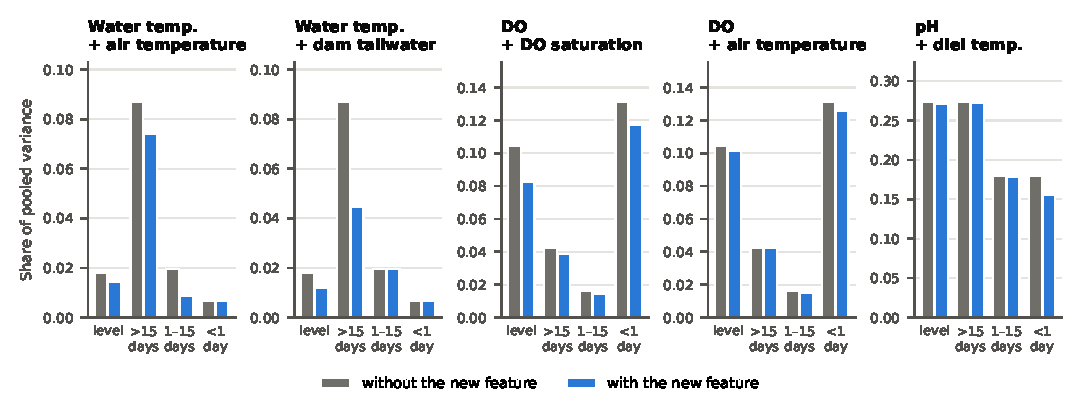
\includegraphics[width=\textwidth]{figures/r2exp_timescales.pdf}
\caption{Graph model error split by time scale, without (gray) and with (blue) the new feature.
Air temperature removes water-temperature error at 1--15 days; tailwater terms remove it at the
seasonal scale; DO saturation removes station-level and sub-daily DO error; the diel term
removes only sub-daily pH error.}
\label{fig:timescales}
\end{figure}

\begin{figure}[h]
\centering
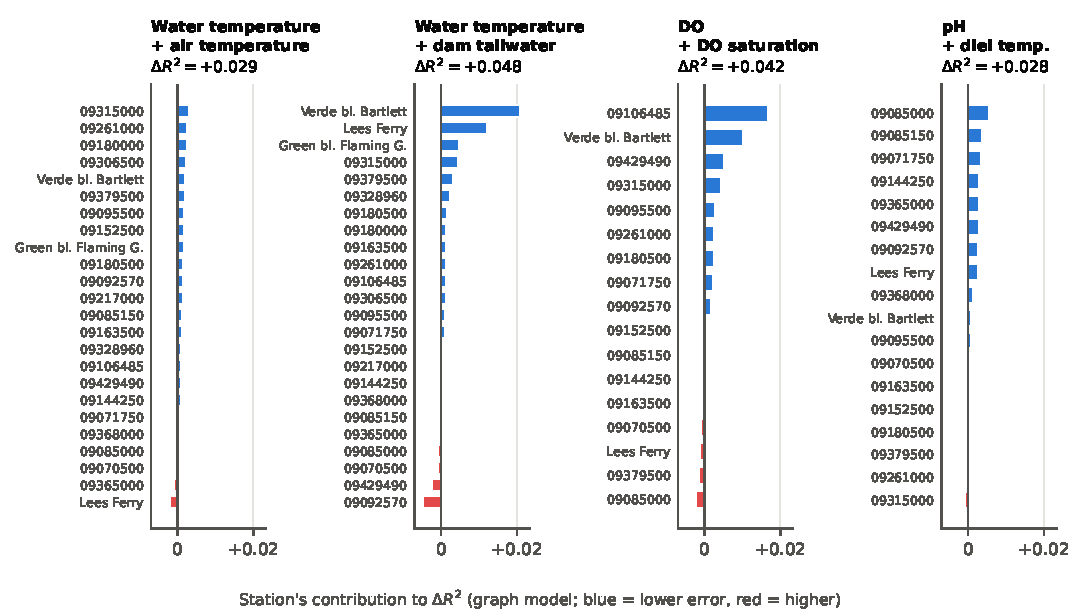
\includegraphics[width=\textwidth]{figures/r2exp_per_station.pdf}
\caption{Each station's contribution to the graph model's $\Delta R^2$ (the contributions add up
to $\Delta R^2$). Air temperature and the diel term help almost every station a little; the
tailwater gain comes mostly from the two tailwater stations, and Lees Ferry, the station air
temperature hurts most, is the one tailwater terms help second most.}
\label{fig:perstation}
\end{figure}

% =====================================================================
\section{Conclusions and next runs}\label{sec:conclusions}

\begin{itemize}
  \item \textbf{Keep three of the four.} DO saturation for DO, air temperature for water
        temperature (and DO, where it adds a little), the diel term for pH. Each gain holds for
        the graph model with an interval that excludes zero, and is spread across stations.
  \item \textbf{Tailwater terms: water temperature only.} They give the largest water-temperature
        gain, but for DO and pH they fail whenever one of the two tailwater stations is held
        out, and they do not help the graph model on specific conductance.
  \item \textbf{Combine air temperature and tailwater for water temperature.} They fix different
        time scales and different stations (air temperature hurts Lees Ferry, which tailwater
        fixes), so they should largely add up: at most about $0.94$ if the gains simply added, somewhat
        less in practice, since both reduce the seasonal part. A paired
        run with both options on is the next experiment, with the tailwater terms offered for
        water temperature only.
  \item \textbf{Keep 19 pH stations.} Setting \code{wt\_diel} to $0$ where a station has no water
        temperature would keep 09371010 and make the pH result comparable with $0.117$.
  \item \textbf{Real-time use.} \code{wt\_diel} uses a centred window; a trailing 24-hour window
        would be needed if the model is ever run in real time.
  \item \textbf{Still running.} The conductance runoff signal for turbidity (with gradient
        boosting) and the graph--GB blend for all five targets will be added when their results
        are in.
\end{itemize}

The new results do not replace the main benchmark numbers on the poster, which were fixed before
these runs.

\end{document}
